\chapter{Conclusiones y resultados}

\section{Algunos resultados}

\begin{figure}[h]
\centering
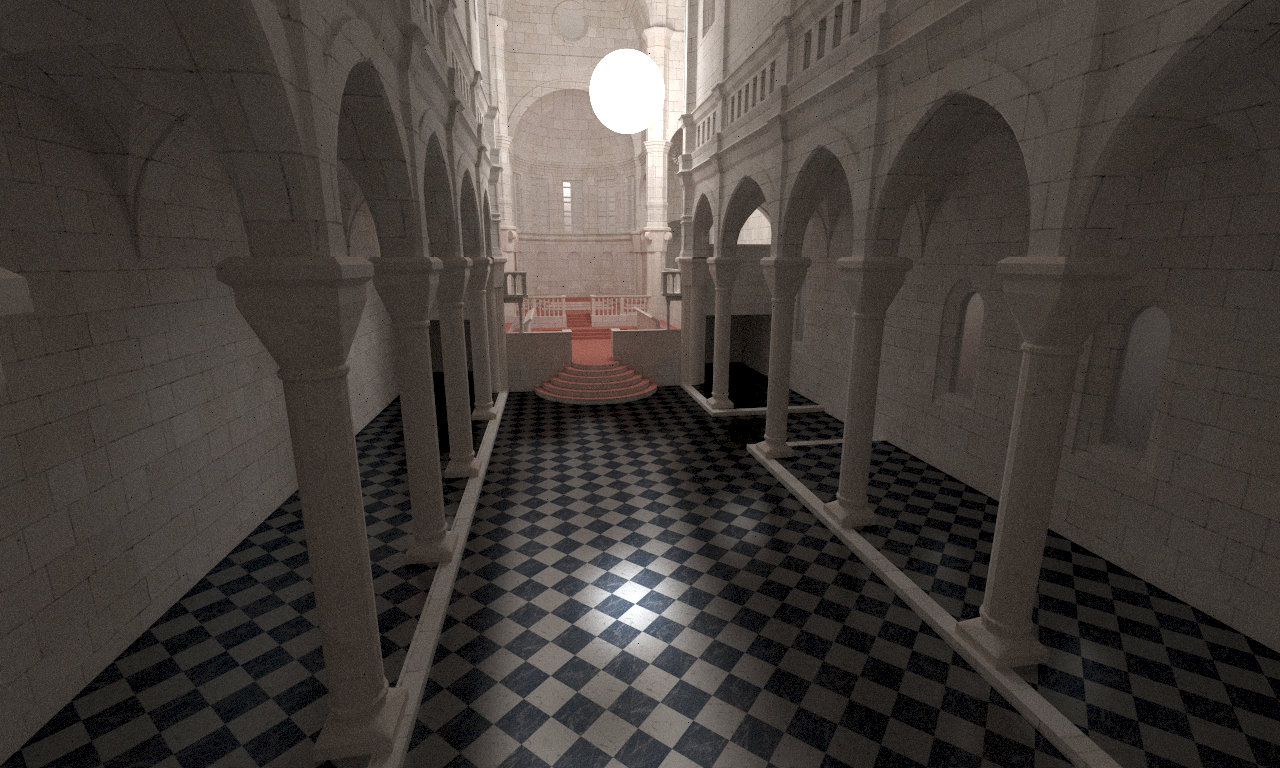
\includegraphics[width=5in]{sibenik_specular.png}
\caption{La textura del suelo es un mapa especular}
\end{figure}

\begin{figure}
\centering
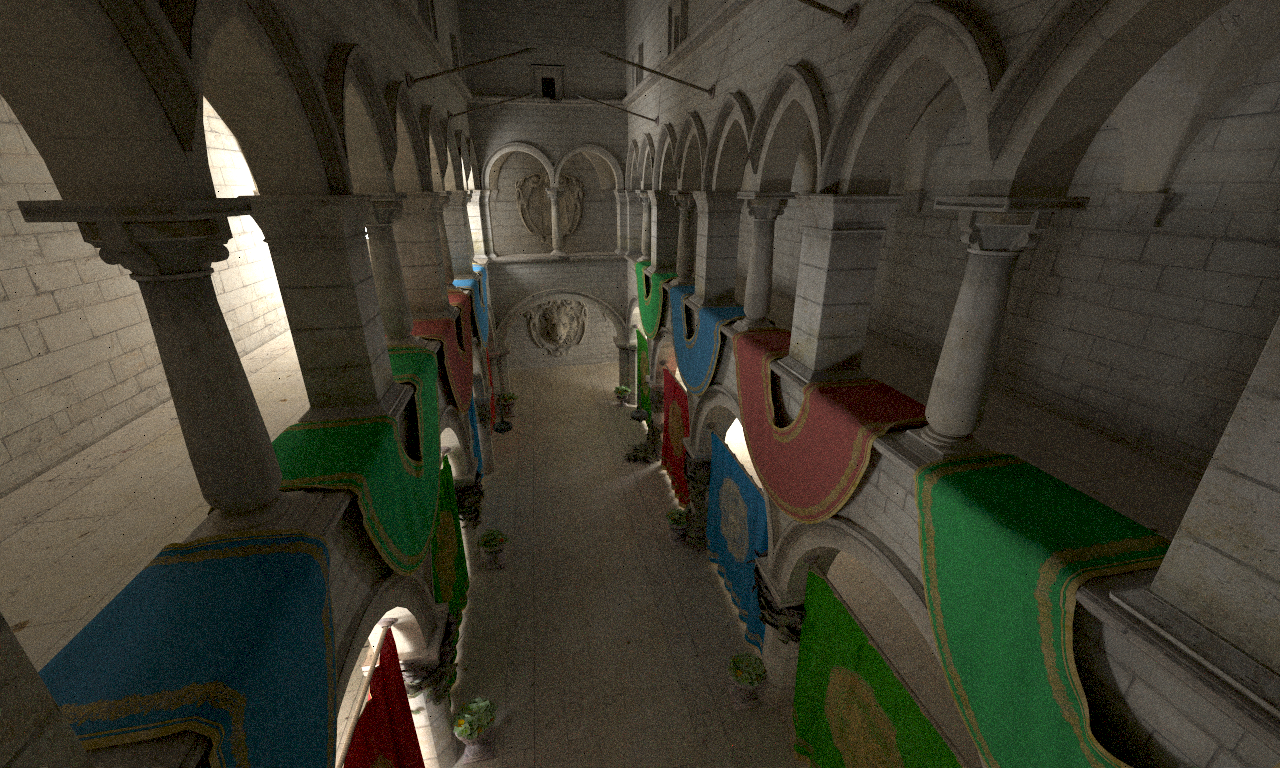
\includegraphics[width=5in]{crytek_sponza1.png}
\caption{Tres fuentes de luz poco visibles iluminan toda la escena}
\end{figure}


\begin{figure}
\centering
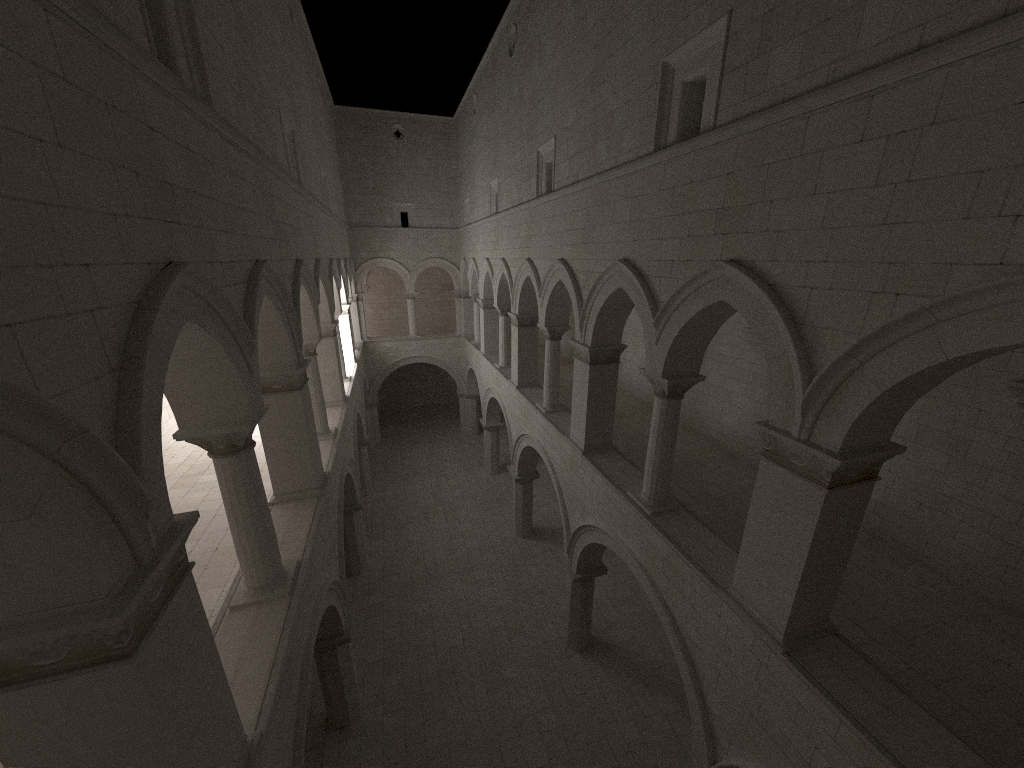
\includegraphics[width=5in]{single_light_sponza.png}
\caption{Iluminación por una única fuente de luz}
\end{figure}

\clearpage

\section{Valoración de los resultados obtenidos}


El campo de estudio en el que se sitúa el presente trabajo es muy amplio y ha sido muy estudiado por un gran número de investigadores. A medida que profundizábamos en la materia de estudio iban surgiendo cada ves más detalles, mejoras y variaciones en la teoría que incrementaban el abasto del proyecto y generaban nuevas dudas. Por ello hemos llegado a un punto en el que, por el alcance de un TFG, hemos tenido que empezar a descartar cosas que al autor le hubiese gustado investigar en más profundidad. Aún así, valoramos positivamente los resultados obtenidos, pues se ha alcanzado el objetivo principal de este trabajo que era implementar un algoritmo de renderizado realista. Además la implementación en la GPU ha demostrado ser bastante rápida, más aún si consideramos que la GPU usada en el desarrollo de este trabajo y en las pruebas realizadas es de una gama baja entre las presentes en el mercado.

\clearpage

\section{Posibles mejoras}

Planteamos tres grupos de posibles mejores bien diferenciados: En primer lugar tenemos las mejoras al algoritmo usado. El algoritmo de path tracing que hemos implementado es una de sus versiones más básicas y tal como hemos comentado en la introducción existen variaciones del mismo que ofrecen mejores resultados en un menor número de muestras. Por ejemplo, una primera mejora seria implementar el transporte de luz bidireccional que ofrecería mejores resultados cuando se trata de iluminar escenas en las que la fuente de luz está muy escondida con respecto a la zona enfocada por la cámara. Otra importante mejora seria explorar e implementar modelos de BRDFs más realistas, pues el que hemos usado es de los más básicos que hay. Además, en este trabajo hemos omitido el importante fenómeno de la refractancia de la luz.

\medskip

Otro grupo de mejoras, más allá de este algoritmo en concreto, sería buscar formas de combinar distintos algoritmos. Aunque en principio el algoritmo utilizado es capaz de simular los fenómenos de la luz más habituales esto no significa que sea el mejor para todos ellos. Existen algoritmos que destacan en simular aspectos específicos del transporte lumínico y un buen motor de renderizado puede aprovechar ese hecho para combinar algoritmos de forma inteligente. Por ejemplo, versiones del algoritmo de radiosity o instant radiosity pueden usarse en una primera fase para computar un mapa de luz difusa de la escena. En una segunda fase se puede utilizar alguna de las variantes de path tracing para calcular la luz especular y la luz refractada, haciendo consultas al mapa de luz difusa cuando sea necesario. Finalmente una ejecución de photon mapping puede usarse para calcular las causticas con un mayor nivel de detalle.
Una buena explicación de este uso combinado de algoritmos se puede encontrar en \cite{Hery2013}.

\medskip

Por último y aunque no era el objetivo de este proyecto, una mejora interesante seria implementar una interfaz de usuario que permitiese configurar la escena de forma fácil y cómoda. Por ejemplo una interfaz con Qt con una vista OpenGL, que permita previsualizar la escena, cargar modelos tridimensionales y colocar las luces y la cámara facilitaría mucho el hecho de configurar escenas y crear nuevos renderizados.

\clearpage

\section{Perspectivas de futuro}

Durante el desarrollo de este proyecto hemos podido comprobar que las ganancias de velocidad al ejecutar el algoritmo de path tracing en la GPU, frente a hacerlo en la CPU, son muy notorias. Con nuestra implementación es posible renderizar escenas de varios millones de polígonos, con cientos de muestras por pixel en unos cuantos minutos. Realizar el mismo tipo de renderizado en una CPU actual podría tardar varios días.

\medskip

Además, considerando que los experimentos se han realizado con una tarjeta gráfica de ordenador portátil y que la implementación es muy optimizable, creemos que en pocos años sera habitual disponer de software capaz de renderizar escenas con iluminación global en tiempo real.

\nocite{Ashikhmin2000}
\nocite{Cook1984}
\nocite{Dutre2003}
\nocite{Torrance1967}
\nocite{Torrance1967}
\nocite{Veach1995}
\nocite{Walter2007}